\documentclass{jib}
\newlength{\platz}
\setlength{\platz}{15pt}
\RequirePackage{listings}
\lstset{%
  basicstyle=\ttfamily,
  fontadjust,
  flexiblecolumns=true,
  frame=L,
  xleftmargin=15pt,
  framesep=5pt,
  emphstyle=\rmfamily\itshape}

\usepackage{pdfpages}

%%%%%%%%%%%%%%%%%%%%%%%%%%%%%%%%%%%%%%%%%%%%%%%%%%%%%%%%%%
% JIB Header/Footer
%%%%%%%%%%%%%%%%%%%%%%%%%%%%%%%%%%%%%%%%%%%%%%%%%%%%%%%%%%
\jibvolume{XX} % insert volume
\jibissue{X}   % insert issue
\jibpages{XXX} % insert article ID
\jibyear{XXXX} % insert year
\makeHeaderFooter{} % leave as is
%%%%%%%%%%%%%%%%%%%%%%%%%%%%%%%%%%%%%%%%%%%%%%%%%%%%%%%%%%

\begin{document}

%%%%%%%%%%%%%%%%%%%%%%%%%%%%%%%%%%%%%%%%%%%%%%%%%%%%%%%%%%
%
% Title Page
%
%%%%%%%%%%%%%%%%%%%%%%%%%%%%%%%%%%%%%%%%%%%%%%%%%%%%%%%%%%

\begin{jibtitlepage}

\jibtitle{The Systems Biology Markup Language (SBML):\\
Language Specification for Level~3 Version~1}

\jibauthor{%
  Ralph Gauges\iref{sigmaringen},
  Ursula Rost\iref{uh},
  Sven Sahle\iref{uh},
  Katja Wengler\iref{uhert},
  Frank T. Bergmann\iref{uh}%
}

\addjibinstitution{sigmaringen}{Hochschule Albstadt-Sigmaringen, Germany}
\addjibinstitution{uh}{University of Heidelberg, Germany}
\addjibinstitution{uhert}{University of Hertfordshire, UK}

\end{jibtitlepage}

% The abstract
\begin{abstract}

  Many software tools provide facilities for depicting reaction network diagrams in a
visual form. Two aspects of such a visual diagram can be distinguished: the layout
(i.e.: the positioning and connections) of the elements in the diagram, and the
graphical form of the elements (for example, the glyphs used for symbols, the
properties of the lines connecting them, and so on).  For software tools that also
read and write models in SBML (Systems Biology Markup Language) format, a common need
is to store the network diagram together with the SBML representation of the model.
This in turn raises the question of how to encode the layout and the rendering of
these diagrams.  The \emph{SBML Level~3 Version~1 Core} specification does not
provide a mechanism for explicitly encoding diagrams, but it does provide a mechanism
for SBML \emph{packages} to extend the Core specification and add additional
syntactical constructs.  The \emph{Layout} package for SBML Level~3 adds the
necessary features to SBML so that diagram layouts can be encoded in SBML files, and
a companion package called SBML \emph{Rendering} specifies how the graphical rendering
of elements can be encoded.

The SBML Layout package is based on the principle that reaction network diagrams
should be described as representations of entities such as species and reactions
(with direct links to the underlying SBML elements), and not as arbitrary drawings
or graphs; for this reason, existing languages for the description of vector drawings
(such as SVG) or general graphs (such as GraphML) cannot be used.


\end{abstract}

% Include your PDF document
%
\includepdf[pages=-]{../spec/sbml-level-3-version-1-core.pdf}
% 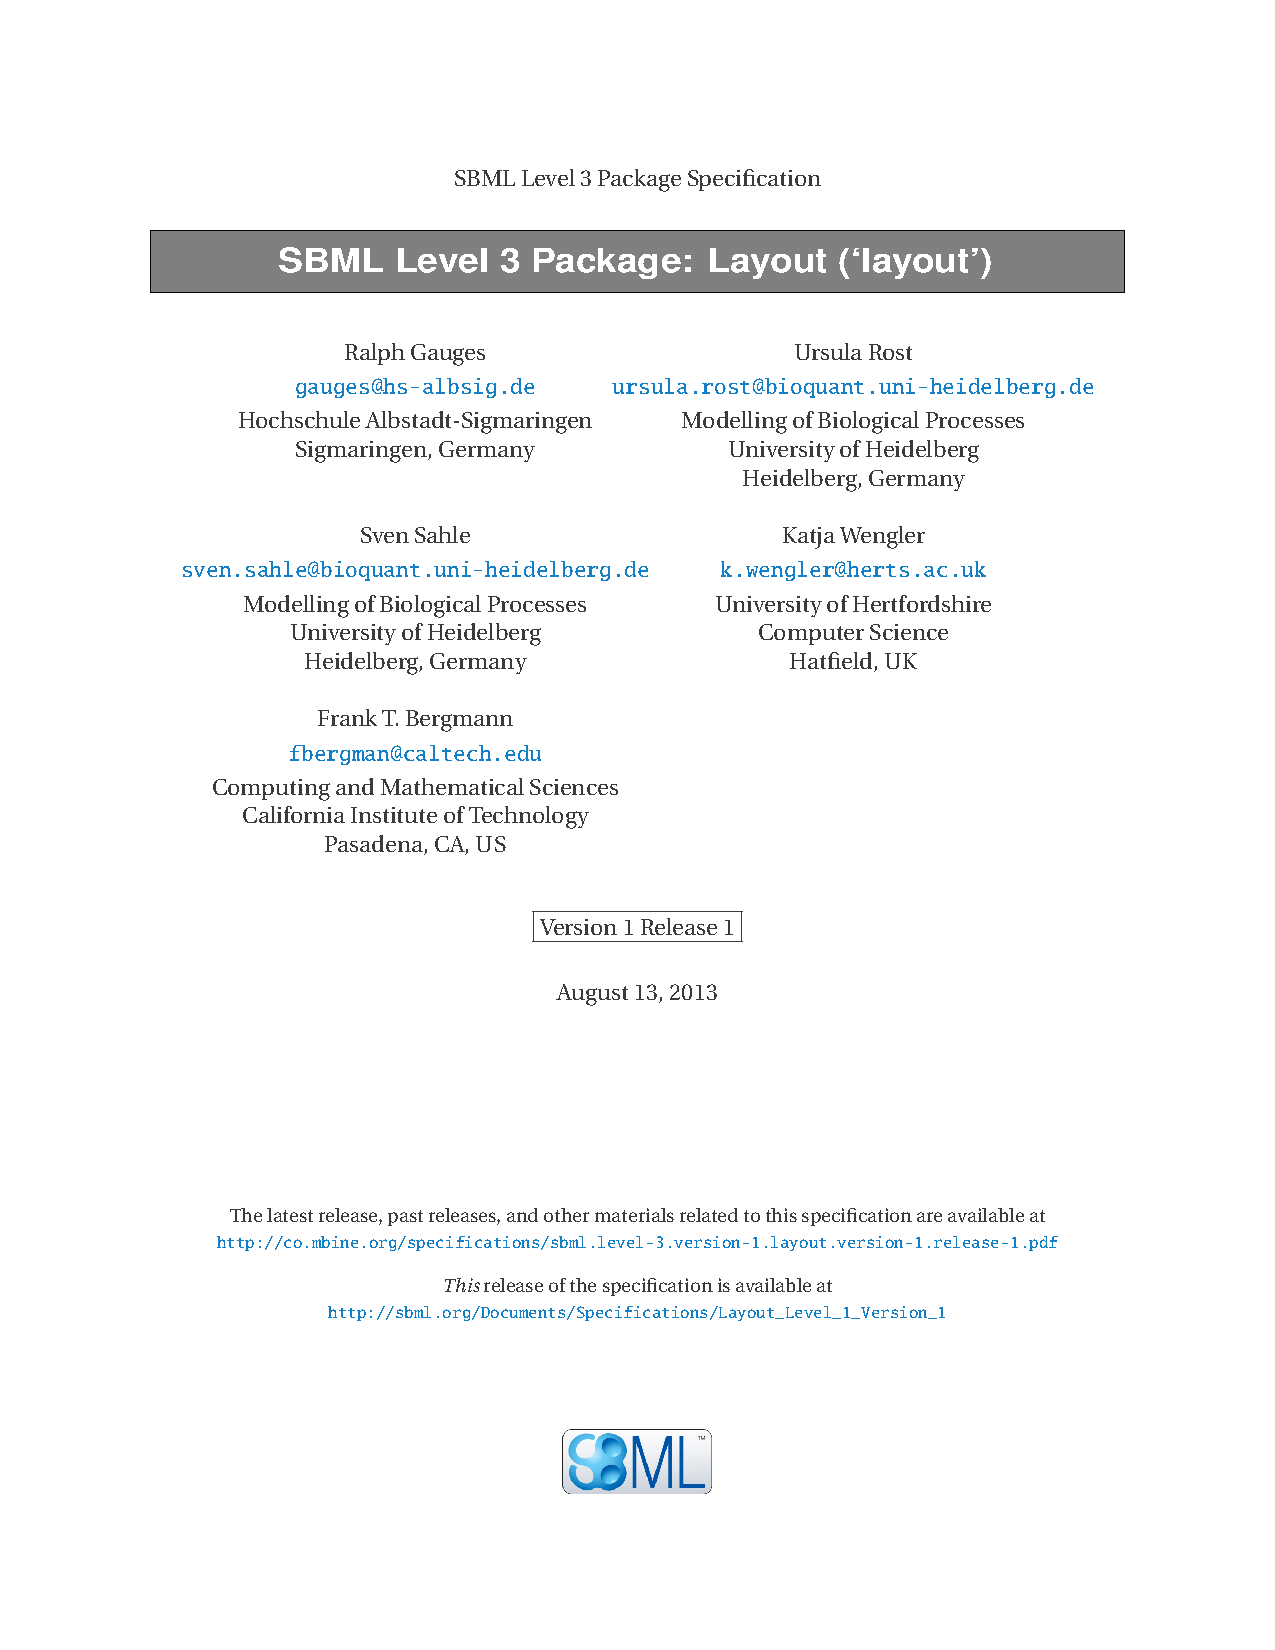
\includepdf[pages=-, offset=0 0, fitpaper=true]{../sbml-layout-version-1-release-1}


\end{document}
